\chapter{Super-Kamiokande Detector Calibration}
\label{chp:superkcalib}


In order to achieve optimal event reconstruction for physics analyses, calibration of the Super-Kamiokande detector is crucial. For example, when constructing Monte Carlo simulations of certain processes in the detector, facets of the experiment such as properties of the water, photomultiplier tube response and the inner detector and outer detector electronics are all calibrated so that input parameters for the Monte Carlo simulations can be obtained. This chapter will concern itself with the inner and outer detector calibration, including photomultiplier tube and electronics calibration, PMT gain calibration, quantum efficiency determination and hit timing and charge information calibration. 

\subsection{Inner detector calibration}
\subsubsection{Electronics and photomultiplier tube calibration}

Understanding the timing information from the hit photomultiplier tubes depends on how well the charge from the hit PMT is calculated. To conceive charge calibration, a quantity called photomultiplier tube ''gain" must be calculated. ''Gain" is the conversion factor from the number of photoelectrons produced by the hit PMT and charge, and calibration of this quantity is what interpretation of very high energy events (TeV scale) rely on. Quantum efficiency is another quantity used for the calibration of low energy physics events (such as detection of solar neutrinos), due to them consisting of single photoelectron (single-pe) hits: it is the ratio of the number of the number of photoelectrons emitted by the cathode to the number of photons that are incident on the photomultiplier tube window. Quantum efficiency is particularly useful for low energy events because the number of photons arriving at the photomultiplier tube window is small. Super-Kamiokande calibration converts this measure of quantum efficiency into ''QE" by multiplying the quantum efficiency by the collection efficiency of the photoelectrons onto the first dynode inside the PMT \ref{abeCalibrationSuperKamiokandeDetector2014}. Knowing the gain and QE of each PMT in the detector is important in order to accurately measure the output charge from each individual PMT, which is done by first calculating the relative gain gain difference among all PMTs and then work out the average gain difference over all PMTs in the detector. After this, the variation away from this average gain value can be calculated for each seperate inner detector photomultiplier tube, and the gain value for each can be extracted. 

The relative gain difference is calculated by two measurements using a light source to produce constant-intensity flashes. The first measurement involves using the light source to produce high-intensity flashes so that all photomultiplier tubes in the detctor gets a certain number of photons, and the second measurement has the light source produce low-intensity flashes so that only a few PMTs are hit. teh first measurement provides an average charge value ($Q_{o b s}(i)$) for each inner detector PMT, while the second measurement gives single photoelectron hits, providing a number of times ($N_{o b s}(i)$) that a single PMT gives a charge which is greater than the PMT threshold value. Equation \ref{eq:gaineq} shows how these two values are calculated from the the high and low intensity flash values ($I$), the acceptance of the PMT(i) ($a(i)$), the QE value of the PMT ($\varepsilon_{q e}$) and the PMT gain $G$. 
****fix this make this equation multiline*******
\begin{equation}
    Q_{o b s}(i) \quad \propto \quad I_{high} \times a(i) \times \varepsilon_{q e}(i) \times G(i)
    \newline
    N_{o b s}(i) \quad \propto \quad I_{low} \times a(i) \times \varepsilon_{q e}(i)
\label{eq:gaineq}
\end{equation}

Therefore, by simply dividing these two values of $Q_{o b s}(i)$ and ($N_{o b s}(i)$) the average gain over all PMTs can be calculated.  Figure \ref{fig:relativegain} shows the spread of the relative gain over all the PMTs. 

\begin{figure}
    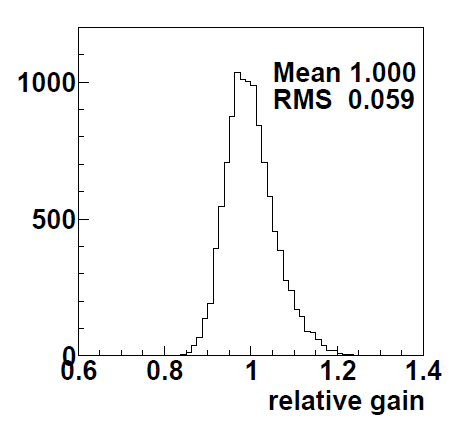
\includegraphics[width=\textwidth]{Figures/relativegain.png}
\caption{Relative gain of PMTs in Super-Kamiokande}
    \label{fig:relativegain}
\end{figure}

